\Section{StreamIt Programming Language}
\label{sec:streamit}

StreamIt~\cite{streamitcc} is an architecture independent language
that is designed for stream programming. In StreamIt, programs are
represented as graphs where nodes represent computation and edges
represent FIFO-ordered communication of data over tapes. The language
features several novelties that are essential for large scale program
development. The language is modular, parameterizable, malleable and
architecture independent. In addition, the language exposes the
inherent parallelism and communication patterns that are prevalent in
streaming programs.

\begin{figure}[t]
  \begin{scriptsize}
	\begin{verbatim}
	  int->int filter ZigZag(int N, int[N] Order) {
	    work pop N push N {
	      for (int i = 0; i < N; i++) {
	        int pixel = peek(Order[i]);
	        push(pixel);
	      }
	      for (int i = 0; i < N; i++) {
	        pop();
	      }
	    }
	  }

	  int[64] Order =
	    {00, 01, 05, 06, 14, 15, 27, 28,
	     02, 04, 07, 13, 16, 26, 29, 42,
	     03, 08, 12, 17, 25, 30, 41, 43,
	     09, 11, 18, 24, 31, 40, 44, 53,
	     10, 19, 23, 32, 39, 45, 52, 54,
	     20, 22, 33, 38, 46, 51, 55, 60,
	     21, 34, 37, 47, 50, 56, 59, 61,
	     35, 36, 48, 49, 57, 58, 62, 63};
	\end{verbatim}
  \end{scriptsize}
  \caption{Zig-zag descrambling filter.}
  \vspace{-12pt}
  \label{fig:zigzag-filter}
\end{figure}

\SubSection{Filters as Programmable Units}
In StreamIt, the basic programmable unit is a {\it filter}.  Each
filter has an independent address space. Thus, all communication with
other filters is via the input and output channels, and occasionally
via control messages (see Section~\ref{sec:messaging}).  The main filter 
method is the work function which represents a steady-state execution step.
The work function pops (i.e., reads) items from the filter input tape
and pushes (i.e., writes) items to the filter output tape. A filter
may also peek at a given index on its input tape without consuming the
item; this makes it simple to represent computation over a sliding
window or to perform permutations on the input stream. The {\tt push},
{\tt pop}, and {\tt peek} rates are declared as part of the work
function, thereby enabling the compiler to apply various optimizations
and construct efficient execution schedules.

A filter is parameterizable,
and this allows for greater malleability and code reuse. An example
filter is shown in Figure~\ref{fig:zigzag-filter}. This filter
consumes a stream whose elements are of type {\tt int} and produces a
stream of the same type. It implements the zig-zag descrambling
necessary to reorder the input stream generated by the run-length
encoding of quantized DCT coefficients. Typically, the zig-zag scan
operates on an 8x8 matrix. Each instantiation of a filter specifies the
matrix dimensions, as well as the desired ordering. In MPEG, there are
two possible scan orders. The {\tt Order} parameter defines the
specific scan pattern that is desired, as shown in 
Figure~\ref{fig:zigzag-filter}.
%% in Figure~\ref{fig:zigzag-filter} implements the default MPEG-2 scan
%% pattern shown in Figure~\ref{fig:zigzag-order}.

In this example, the input matrix is represented as a unidimensional
stream of elements. The filter peeks the elements and
copies them to the output stream in the specified order. Once all the
DCT coefficients are copied, the input stream is deallocated from the
tape with a series of pops.  It has been shown that vector permutation
instructions can be automatically generated from this
representation~\cite{yelick04msp}.

\begin{figure}[t]
  \center{
 	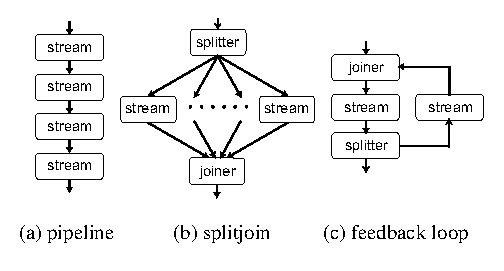
\includegraphics[scale=1, angle=0]{./constructs-eg.eps}
 	\caption{Hierarchical streams in StreamIt.}
%    \vspace{-12pt}
 	\label{fig:containers}
  }
\end{figure}

\begin{figure}[t]
  \begin{scriptsize}
    \begin{verbatim}
      int->int pipeline InverseTransform() {
        int[64] Order = {...};
        add ZigZag(64, Order);
        add IQuantization(64);
        add IDCT(64);
        add Saturation(64);
      }
    \end{verbatim}
  \end{scriptsize}
  \caption{Example pipeline.}
%  \vspace{-12pt}
  \label{fig:decoder-pipeline}
\end{figure}

\SubSection{Hierarchical Streams}
In StreamIt, the application developer focuses on the hierarchical
assembly of the stream graph and its communication topology, rather
than the explicit management of the data buffers between filters.
StreamIt provides three hierarchical structures for composing filters
into larger stream graphs (see Figure~\ref{fig:containers}).

\paragraph{Pipeline.}
A StreamIt pipeline is a parameterized stream that composes streams in
sequence, with the output of one connected to the input of the next.
An example of a pipeline appears in
Figure~\ref{fig:decoder-pipeline}. A pipeline is a single input to
single output stream. The decoding pipeline in the figure consists of
four streams. The first is a filter which zig-zag unorders the input
stream, preparing the data for the inverse quantization and
DCT. The output of the filter is consumed by a stream named {\tt
IQuantization} that performs the inverse quantization, and produces an
output stream that is in turn consumed by another stream that performs
the inverse DCT.

The {\tt add} keyword in StreamIt constructs the specified stream
using the input arguments. The {\tt add} statement may only appear in
non-filter streams.  In essence, filters are the leaves in the
hierarchical construction, and composite nodes in the stream graph
define the encapsulating containers. This allows for modular design
and development of large applications, thereby  promoting
collaboration, increasing code reuse, and simplifying debugging.

\paragraph{Split-Join.}
The splitjoin construct distributes data to a set of parallel
streams, which are then joined together in a roundrobin fashion. In a
splitjoin, the {\it splitter} performs the data scattering, and the
{\it joiner} performs the gathering. A splitter is a specialized
filter with a single input and multiple output channels. On every
execution step, it can distribute its output to any one of its
children in either a {\it duplicate} or a {\it roundrobin} manner.  A
duplicate splitter (indicated by \texttt{split duplicate}) replicates
incoming data to each stream connected to the splitter.  A
roundrobin splitter (indicated by {\tt split
roundrobin($w_1,\ldots,w_n$)}) distributes the first $w_1$ items to
the first child, the next $w_2$ items to the second child, and so
on.  The splitter counterpart is the joiner. 
%% It is a specialized
%% filter with multiple input channels but only one output
%% channel. The joiner
It gathers data from its predecessors in a roundrobin manner to
produce a single output stream.

\begin{figure}[t]
  \begin{scriptsize}
    \begin{verbatim}
      float->float pipeline IDCT_2D(int N) {
        // perform N 1D-IDCTs in parallel in the X direction
        add splitjoin {
          split roundrobin(N);
          for (int i = 0; i < N; i++)
            add IDCT_1D(N);
          join roundrobin(N);
        }
        // perform N 1D-IDCTs in parallel in the Y direction
        add splitjoin {
          split roundrobin(1);
          for (int i = 0; i < N; i++)
            add IDCT_1D(N);
          join roundrobin(1);
        }
      }

      float->float filter IDCT_1D(int N) {
        float[N][N] coeff = { ... };
        
        work pop N push N {
          for (int x = 0; x < N; x++) {
            float product = 0;
            for (int u = 0; u < N; u++)
                product += coeff[x][u] * peek(u);
            push(product);
          }
          for (int x = 0; x < N; x++) pop();
        }
      }
    \end{verbatim}
  \end{scriptsize}
  \caption{Example MPEG decoder splitjoin.}
%  \vspace{-12pt}
  \label{fig:decoder-sj}
\end{figure}

\begin{figure}[t]
  \begin{scriptsize}
    \begin{verbatim}
      // global variable
      float coeff[64] = { ... };
      
      void IDCT_2D(float* block) {
        int i, j, u;
        float product;
        float tmp[64];
        
        // 1D DCT in X direction
        for (i = 0; i < 8; i++)
          for (j = 0; j < 8; j++) {
            product = 0;

            for (u = 0; u < 8; u++)
              product += c[u][j] * block[8*i + u];

            tmp[8*i + j] = product;
          }

        // 1D DCT in Y direction
        for (j = 0; j < 8; j++)
          for (i = 0; i < 8; i++) {
            product = 0;

            for (u = 0; u < 8; u++)
              product += c[u][i] * tmp[8*u + j];

            block[8*i + j] = product;
          }
      }
    \end{verbatim}
  \end{scriptsize}
  \vspace{-12pt}
  \caption{Example C code for 2D inverse DCT calculation using two 1D transforms.}
  \label{fig:idct_creference}
\end{figure}

The splitjoin and pipeline constructs provide a convenient and natural
way to represent parallel computation. An example is shown in
Figure~\ref{fig:decoder-sj}, which illustates a parallel
implementation of the 2D inverse DCT using 1D inverse DCTs. This
implementation is both data parallel (within the rows and columns) and
pipeline parallel (between the rows and columns). 
A straightforward C implementation of a computationally equivalent
inverse DCT is shown in Figure~\ref{fig:idct_creference}. Note that
the code structure is similar to the StreamIt version, although it does 
not explicitly expose the parallelism.
The C code also requires explicit array index management, such as the 
expressions \texttt{block[8*i + u]} and \texttt{tmp[8*i + j]} which are
notably absent in the StreamIt code. 
The splitter and joiner in StreamIt free the programmer from
tedious indexing operations, which also enables the compiler to
understand and optimize the buffer management~\cite{sermulins05lctes}.
The StreamIt implementation is also parameterized such that it is
trivial to adjust the size of the inverse DCT.

%% For example, when the decoder performs the
%% luminance and chrominance channel processing, the computation can
%% occur in parallel. In StreamIt, this is expressed as shown in
%% Figure~\ref{fig:decoder-sj}. The input stream contains the
%% macroblock data along with the parsed motion vectors. The data is
%% partitioned and passed to one of three decoding channels, with $4N$
%% items assigned to the first stream, $N$ items to the second, and $N$
%% items to the third. The three streams reconstruct the original
%% pictures with respect to the different color channels, and their
%% output is combined by the joiner to produce the final decoded picture.

\paragraph{Feedback Loop.}
StreamIt also provides a feedback loop construct for introducing
cycles in the graph. This stream construct is not used in the decoder,
but may be used in the MPEG encoder.

\SubSection{Teleport Messaging}
\label{sec:messaging}
A notoriously difficult aspect of stream programming, from both a
performance and programmability standpoint, is reconciling regular
streaming dataflow with irregular control messages.  While the
high-bandwidth flow of data is very predictable, realistic
applications such as MPEG also include unpredictable, low-bandwidth
control messages for adjusting system parameters (e.g., desired
precision in quantization, type of picture, resolution, etc.).

For example, the inverse quantization step in the decoder uses a
lookup table that provides the inverse quantization scaling factors.
However, the particular scaling factor is determined by the stream
parser. Since the parsing and inverse quantization tasks are logically
decoupled, any pertinent information that the parser discovers must be
forwarded to the appropriate streams.  In StreamIt, such
communication is conveniently accomplished using teleport
messaging~\cite{thies05ppopp}.

The idea behind teleport messaging is for the {\tt Parser} to change
the quantization precision via an asynchronous method call, where
method invocations in the target are timed relative to the flow of
data in the stream (i.e., macroblocks). As shown in
Figure~\ref{fig:messaging}, the {\tt InverseDCQuantizer} declares a
message handler that adjusts its precision (lines 27-29). The {\tt
Parser} calls this handler through a {\it portal} (line 16), which
provides a clean interface for messaging.  The handler invocation
includes a range of latencies {\tt [min:max]} specifying when the
message should be delivered with respect to the data produced by the
sender.

Intuitively, the message semantics can be understood as tags
attached to data items.  If the {\tt Parser} sends a message to
a filter downstream (i.e., in the same direction as dataflow) with a
latency $k$, then, conceptually, the filter tags the items that it
outputs in $k$ iterations of its work function. If $k=0$, the data
produced in the current execution of the work function is tagged. The
tags propagate through the stream graph; whenever a filter inputs an
item that is tagged, all of its subsequent outputs are also
tagged. The message flows through the graph until the first tagged data
item reaches the intended receiver, at which time the message handler is
invoked immediately before the execution of the work function in the
receiver.  In this sense, the message has the semantics of traveling
``with the data'' through the stream graph, even though it is not
necessarily implemented this way.

%% The intuition for upstream messages is somewhate similar. Namely,
%% immagine a feedback loop connecting the downstream sender with the
%% upstream message receiver. The downstream filter uses the loop to send
%% tokens on every iteration, and the upstream filter checks the values
%% from the loop before each of its executions. If the value is non-zero,
%% it is treated as a message, otherwise the token is ignored. In this
%% scenario, the upstream message is processed immediately before it
%% generates data that the sender will consume in $k$ of its own
%% iterations.

Teleport messaging avoids the muddling of data streams with
control-relevant information. Teleport messaging thus separates the
concerns of the programmer from the system implementation,
thereby allowing the compiler to deliver the message in the most
efficient way for a given architecture. In addition, by exposing the
exact data dependences to the compiler, filter executions can be
reordered so long as they respect the message timing.  Such reordering
is generally impossible if control information is passed via global
variables.  Teleport messaging also offers other powerful control over
timing and latency beyond what is used in this example (in particular,
the ability to send messages opposite the direction of
dataflow~\cite{thies05ppopp}).

\begin{figure}[t]
  %\center{
  %\begin{minipage}[t]{3.8in}
  %{
  %\vspace{-180pt}
  \begin{scriptsize}
    \begin{verbatim}
	01 void->void MPEGDecoder {
	02   ...
	03   portal<InverseDCQuantizer> p;
	04   ...
	05   add Parser(p);
	06   ...
	07   add InverseDCQuantizer() to p;
	08   ...
	09 }

	10 int->int filter Parser(portal<InverseDCQuantizer> p) {
	11   work push * {
	12     int precision;
	13     ...
	14     if (...) {
	15       precision = pop();
	16       p.setPrecision(precision) [0:0];
	17     }
	18     ...
	19   }
	20 }

	21 int->int filter InverseDCQuantizer() {
	22   int[4] scalingFactor = {8, 4, 2, 1};
	23   int    precision = 0;

	24   work pop 1 push 1 {
	25     push(scalingFactor[precision] * pop());
	26   }

	27   handler setPrecision(int new_precision) {
	28     precision = new_precision;
	29   }
	30  }
    \end{verbatim}
  \end{scriptsize}
  %\vspace{-3pt}
  %}
  %\end{minipage}
  %~~\vrule~~
  %\begin{minipage}[t]{2.8in}
  %{
  %  \vspace{50pt}
  %  \center{
  %	    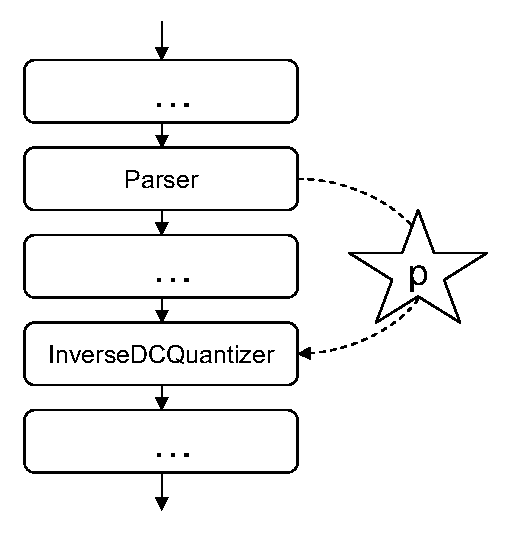
\includegraphics[scale=.9, angle=0]{./messaging_example_fig.eps}
  %  }
  %}
  %\end{minipage}
  %}
  \caption{MPEG messaging example.}
  \label{fig:messaging}
\end{figure}
